\chapter{Goals}
\label{chap:goal}

\section{Project objectives}

Not long after the COVID-19 pandemic started, people realized that the disease could spread by means of water droplets suspended in the air.
This lead many research groups in the fluid dynamics domain to investigate how air would move inside a room, carrying such droplets (some examples:~\cite{covid-air-1}\cite{covid-air-2}).

The overall project that includes my thesis is a research topic on this momentum.
The final goal is to understand the common patterns that air follows when moving --- while apparently being still --- in a room.
To understand this, an experimental setup was created in a small room.
In a corner of the chamber there was a machine~\cite{bubble-machine} able to create bubbles, similar in concept to the soap bubbles that children use to play (figure~\ref{fig:experimetal-setup}). By observing the movement of these bubbles, the movement of the air would then be inferred.

Since the bubbles need to move in the same way of the surrounding air, a way to cancel out all the other forces is required.
The surface and filling material for the bubbles therefore need to be carefully chosen, in order to have an overall weight density of the bubble similar to the air density.
This allows the buoyancy force to compensate almost exactly the gravity force, leaving only the force of the surrounding air to move the bubble.

The experiments are conducted in two steps.
First, some bubbles are created: when there are enough, the machine is stopped, to avoid air currents caused by the machine itself.
Then, a small amount of time is waited, to allow the bubbles to lose their initial speed, and to settle in the room air movement.
After this this short period, the observation starts.
Due to this composed procedure, the ``bubble material'' would be required to create long-lasting bubbles, whose average lifetime is at least 5 minutes.

On top of that, soap bubbles are too big for the purpose: there is a high chance that a bubble in front occludes another bubble in the back, reducing the quality of the observation.
For this reason, the ``soap'' must be a material that creates bubbles with a maximum diameter of some millimeters.

From all these considerations, the bubbles were created with a coating made of a proprietary substance created by Sage Action~\cite{bubble-substance}, filled with helium.

\begin{figure}
	\centerline{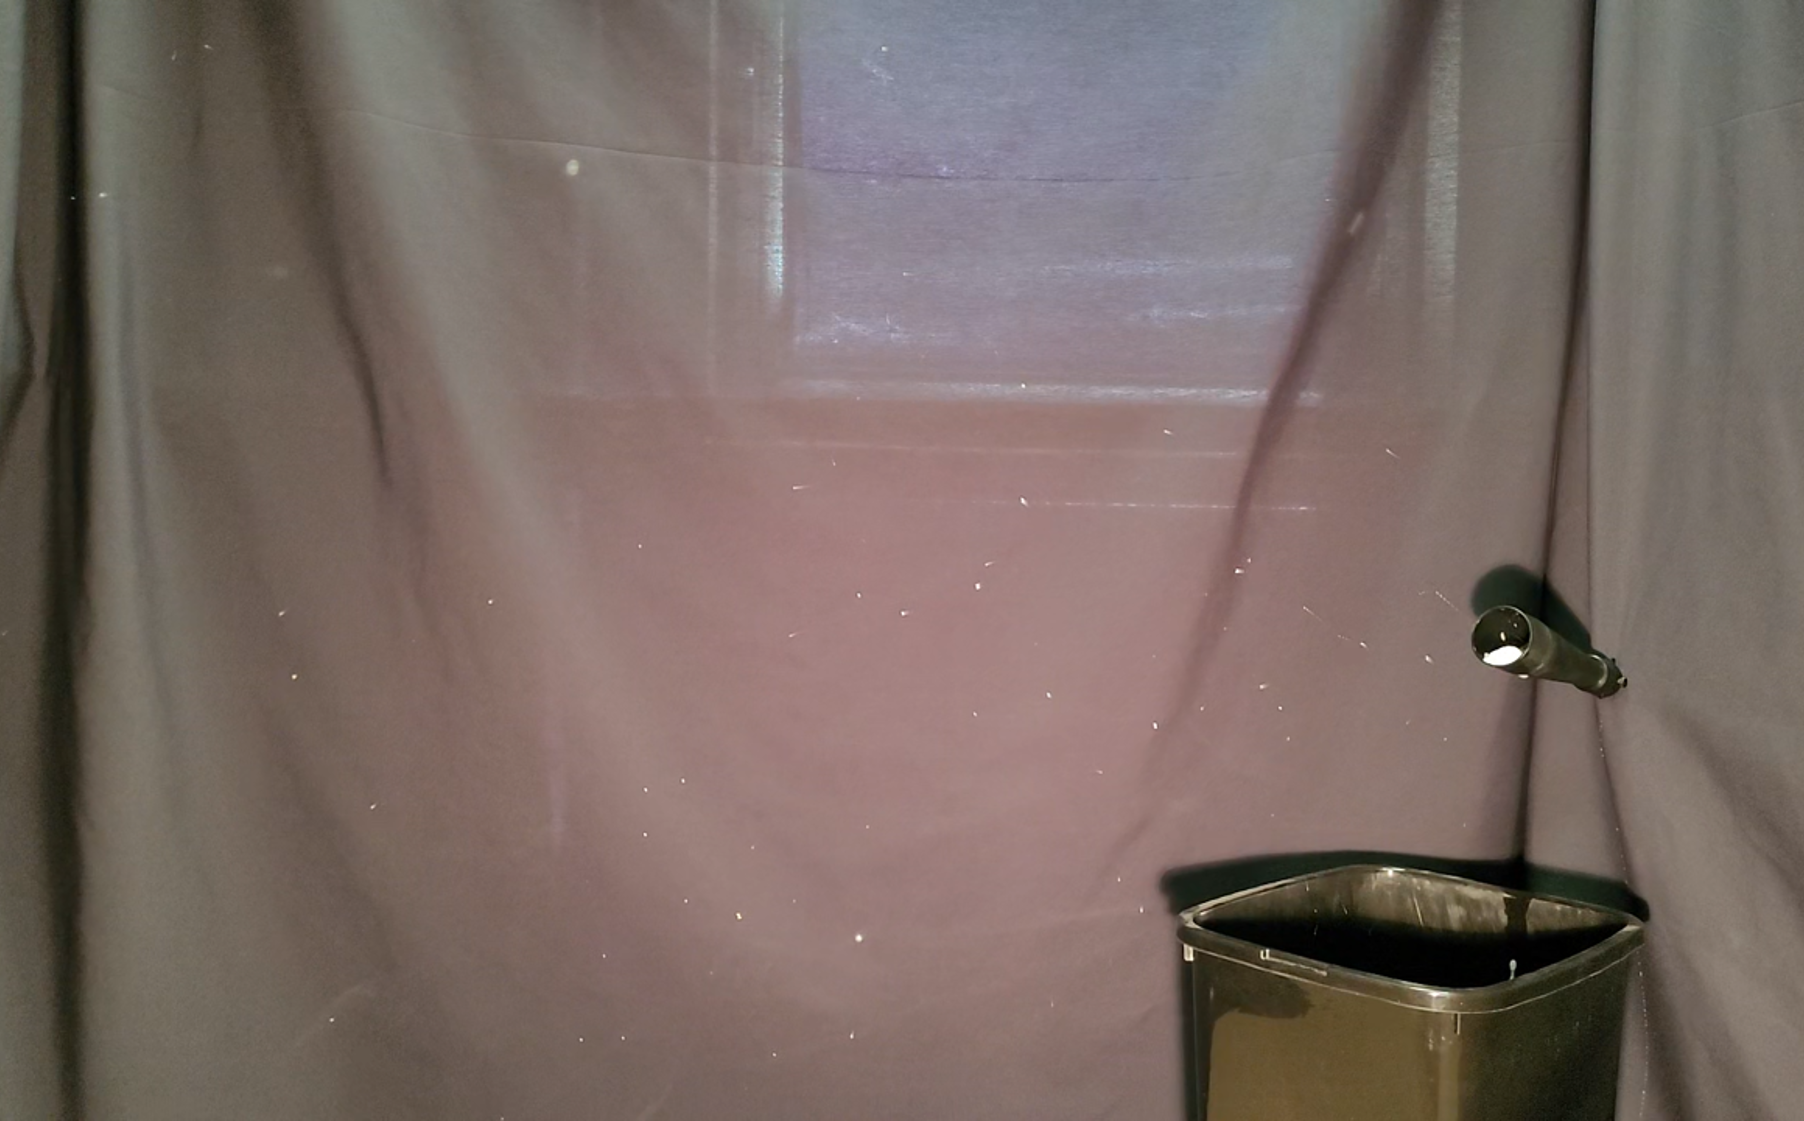
\includegraphics[width=0.9\textwidth]{images/experimental-setup.png}}
	\caption{\centering The experimental setup: the machine in the corner of the room is creating some small bubbles that fill the space}
	\label{fig:experimetal-setup}
\end{figure}

\section{Company objectives}

\subsection{The cameras}

SMA-RTY France~\cite{smarty-website}, the company where I did my internship, has as core business the selling of special-purpose, FPGA-driven cameras.
As such, one of the two tasks contracted to them by the research group was the construction of a specific camera for this purpose: this task was tackled by their internal team of embedded developers.
In the final setup, 3 or 4 cameras were used in a stereoscopic arrangement, as shown in figure~\ref{fig:camera-setup}.

\begin{figure}
	\centerline{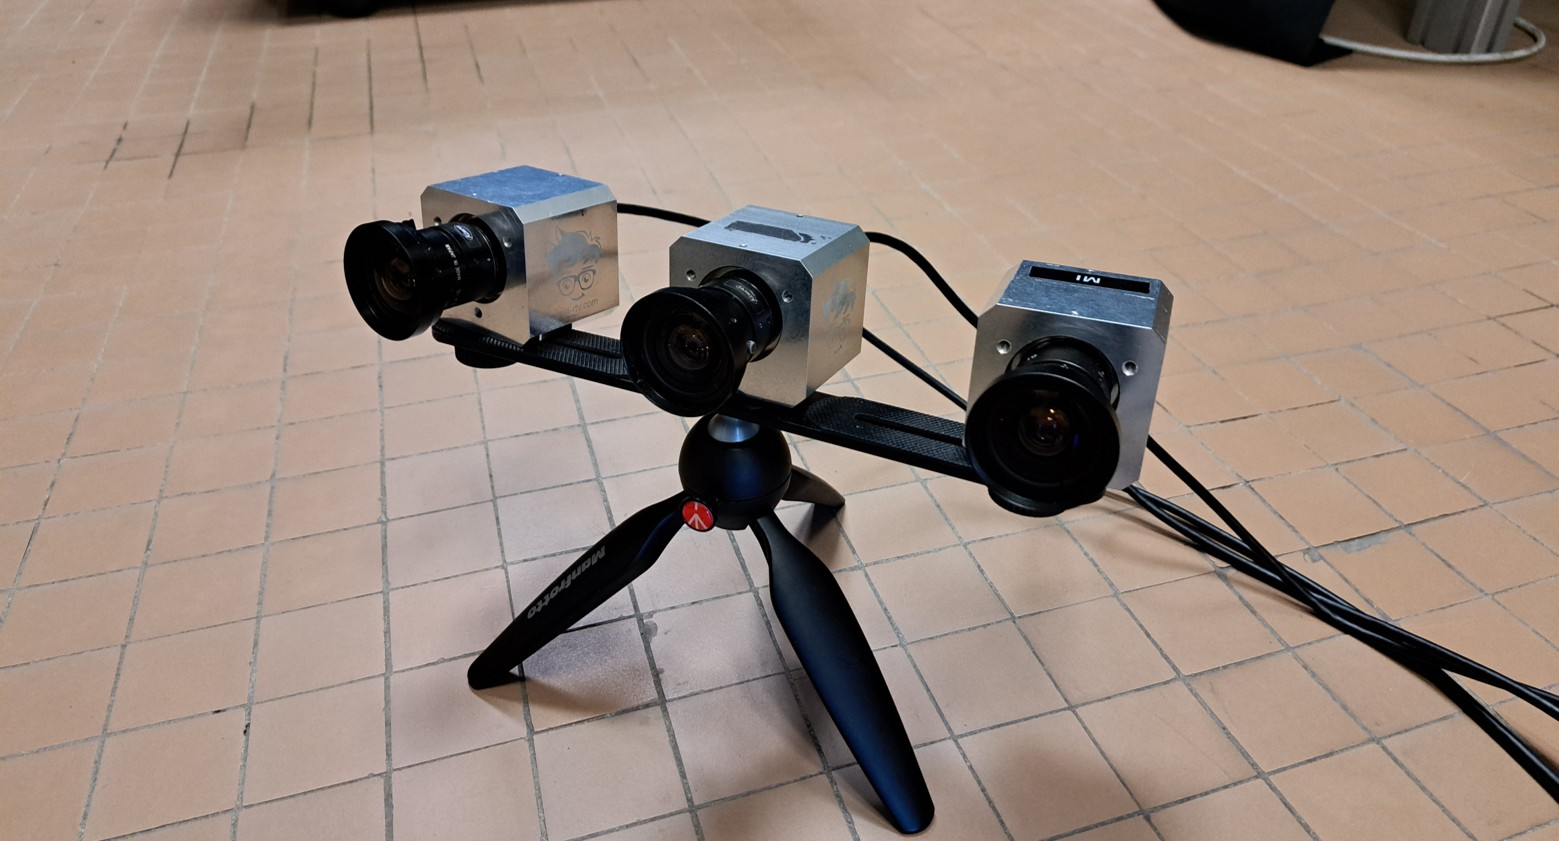
\includegraphics[width=0.9\textwidth]{images/cameras.jpg}}
	\caption{\centering A tripod with 3 SMA-RTY cameras in a stereoscopic arrangement}
	\label{fig:camera-setup}
\end{figure}

\subsection{Reconstruction algorithm acceleration}

The research group internally developed a Matlab tool for analyzing the video footage from an arrangement of 3 cameras, but the processing speed was extremely slow.
As such, they contracted SMA-RTY to create an accelerated version, either by improving the original one, or by creating a totally new script, in whichever programming language was best.
The objective of the acceleration was to have a real-time software, that would be able to process the videos live, with an allowance of some seconds of jitter.
That is, a delay between capturing the frame and outputting the reconstruction was acceptable, as long as it did not increase over time.

SMA-RTY internally started working on this, with a different solution that accelerated the processing to 19 FPS.
This script was already orders of magnitude faster than the original one, but the obtained speed was still less than the target.
On top of this, this proposed solution was working with ToF (Time of Flight) cameras to perform the depth estimation, thus avoiding the expensive 3D reconstruction methods.
However, the project required visible cameras, therefore this idea had to be discarded.

\section{Thesis objectives}

I was assigned by the SMA-RTY team the task of accelerating the Matlab script for processing the videos.
Originally, the vision was to exploit my CUDA skills to leverage the parallelization of GPUs.
However, as the body of this thesis will make clear, there was not so much parallelization that could be done.
Instead of focusing on ``better'' hardware architectures, the best course of action was indeed to optimize the various software steps.

Therefore, the objective of my thesis became the recreation of the full pipeline, from image capturing to 3d markers rendering.
The main constraint of the result would be the speed, 24 FPS were required at steady-state, while the output quality should be as good as possible.
